\documentclass[tikz,border=3pt]{standalone}
\usepackage[utf8]{inputenc}
\usepackage[T1]{fontenc}
\usepackage{lmodern}
\renewcommand{\familydefault}{\sfdefault}
\usepackage{sansmath}\sansmath
\usepackage{chemfig}
\usepackage{pgfplots}\pgfplotsset{compat=1.18,/pgf/number format/use comma,/pgf/number format/1000 sep={.}}
\usetikzlibrary{arrows.meta,calc,positioning,decorations.pathmorphing,patterns}
% paleta del sitio
\definecolor{nar}{HTML}{E8680C}\definecolor{narc}{HTML}{FFB35C}\definecolor{hielo}{HTML}{FFF3E8}
\definecolor{tinta}{HTML}{1D1D1F}\definecolor{gris}{HTML}{6E6E73}\definecolor{lila}{HTML}{7C5CF0}
\definecolor{azul}{HTML}{2F6FD6}\definecolor{menta}{HTML}{17A673}\definecolor{coral}{HTML}{E8342A}
\begin{document}
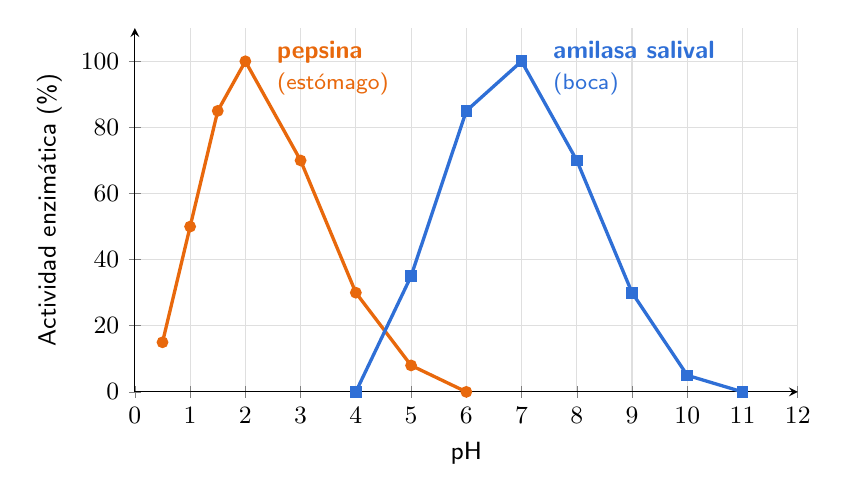
\begin{tikzpicture}[font=\small]
\begin{axis}[width=10cm,height=6.2cm,axis lines=left,xmin=0,xmax=12,ymin=0,ymax=110,xtick={0,1,...,12},ytick={0,20,...,100},
  grid=major,grid style={gray!25},xlabel={pH},ylabel={Actividad enzimática (\%)},clip=false]
\addplot[nar,very thick,mark=*,mark options={fill=nar,scale=0.75}] coordinates {(0.5,15)(1,50)(1.5,85)(2,100)(3,70)(4,30)(5,8)(6,0)};
\addplot[azul,very thick,mark=square*,mark options={fill=azul,scale=0.75}] coordinates {(4,0)(5,35)(6,85)(7,100)(8,70)(9,30)(10,5)(11,0)};
\node[nar,font=\small\bfseries,anchor=west,align=left] at (axis cs:2.4,98) {pepsina\\{\footnotesize\mdseries (estómago)}};
\node[azul,font=\small\bfseries,anchor=west,align=left] at (axis cs:7.4,98) {amilasa salival\\{\footnotesize\mdseries (boca)}};
\end{axis}
\end{tikzpicture}
\end{document}
